\documentclass[extendedabs]{bmvc2k}
\usepackage[ruled]{algorithm2e}
\begin{document}

\section*{digital image processing hw2}
\subsection*{problem 1: guided filter}

Guided filter \cite{guided} is an explicit image filter which have the edge-preserving 
smoothing property like the bilateral filter, but also handles gradient reversal artifacts
within O($N$) time complexity where N is the number of pixels.

In joint bilateral filter, input image can be smoothed with the help of a guidance image,
resulting more reliable smoothing regarding the precise edge components. However,
bilateral filter suffers from the gradient reversal artifacts because the pixels around
the edge has high intensity variance which makes the averaged output unreliable. 
Furthermore, the naive implementation of the bilateral filter elapses O($Nr^2$) time, 
which is impractical when kernel radius $r$ is large.

In guided filter, filter output is assumed to be a linear transformation of guidance $I$
with linear coefficients $a_k$, $b_k$ in a window $\omega_k$ of center pixel $k$.
Coefficients are optimized to minimize the difference between filter output $q$ and input $p$:
\[E(a_k,b_k) = \sum_{i \in \omega_k}((a_kI_i + b_k - p_i)^2 + \epsilon a_k^2)\]
which can be solved by linear regression to have each coefficients as:
\[a_k=\frac{1/|\omega|\sum_{i \in \omega_k}I_ip_i - \mu_k\bar{p_k}}{\sigma_k^2+\epsilon}\]
\[b_k=\bar{p_k} - a_k\mu_k\]
where $\mu_k$, $\sigma_k^2$ are the mean, variance of $I$ in $\omega_k$, 
$\bar{p_k}=1/|\omega|\sum_{i \in \omega_k}p_i$.
$\epsilon a_k^2$ is a regularization term to prevent explosion of $a_k$.
Moreover, low-pass filter can be approximated when $\sigma_k^2 << \epsilon$ and thus
$a_k \sim 0$, $b_k \sim \bar{p_k}$.

When applying the window in the image, several windows $\omega_k$ can affect a same pixel $i$.
Thus output $q_i$ can be averaged from all the possible windows $\omega_k$ in which the pixel $i$
is within the window:
\[q_i = 1/|\omega|\sum_{k:i \in \omega_k}(a_kI_i + b_k)\]

From the equation above, it can be found that box filters ($\sum_{i \in \omega_k}f_i$) are 
the only filters applied in calculating the output image. 
Thus by using the integral image technique, 
the time complexity of guided filter becomes O($N$) where N is the number of pixels.

\begin{figure}[h]
    \centering
    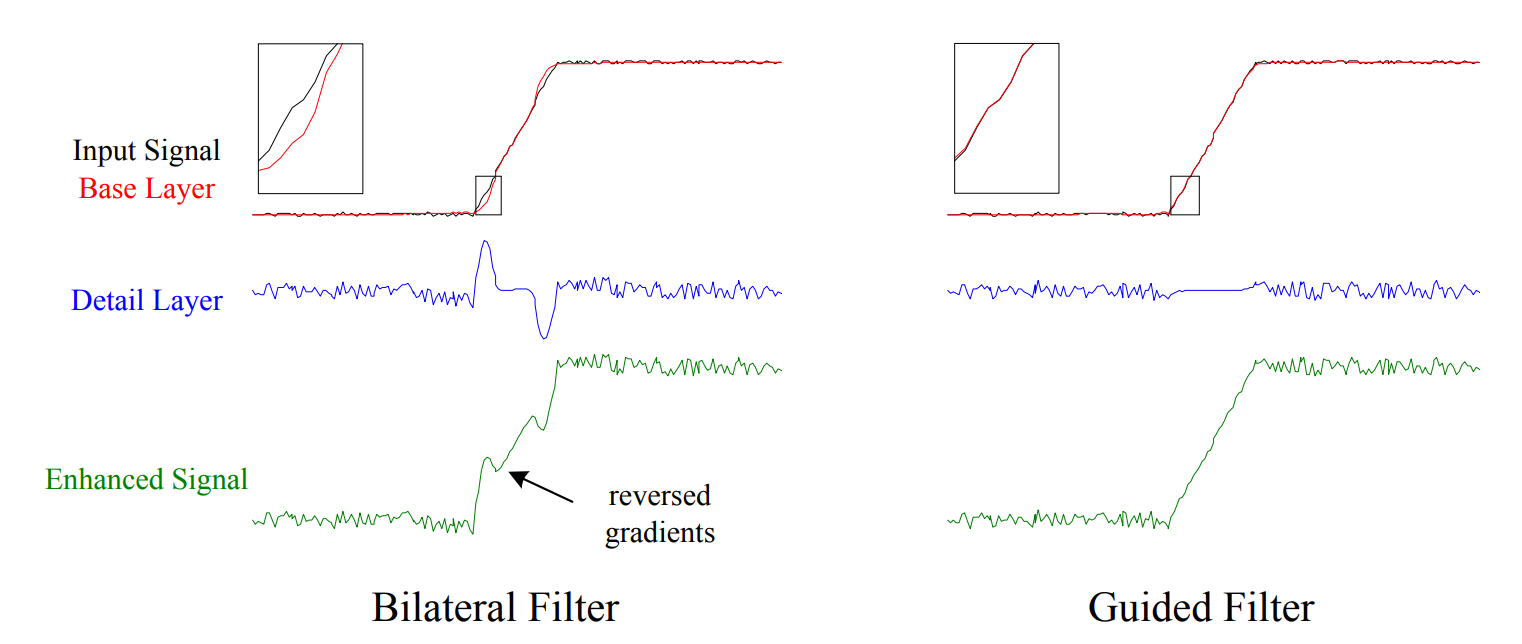
\includegraphics[width=\linewidth]{hw2_1_1}
    \caption{gradient reversal effect from bilateral filter and the corresponding guided filter result}
    \label{fig:1}
\end{figure}

\begin{figure}[h]
    \centering
    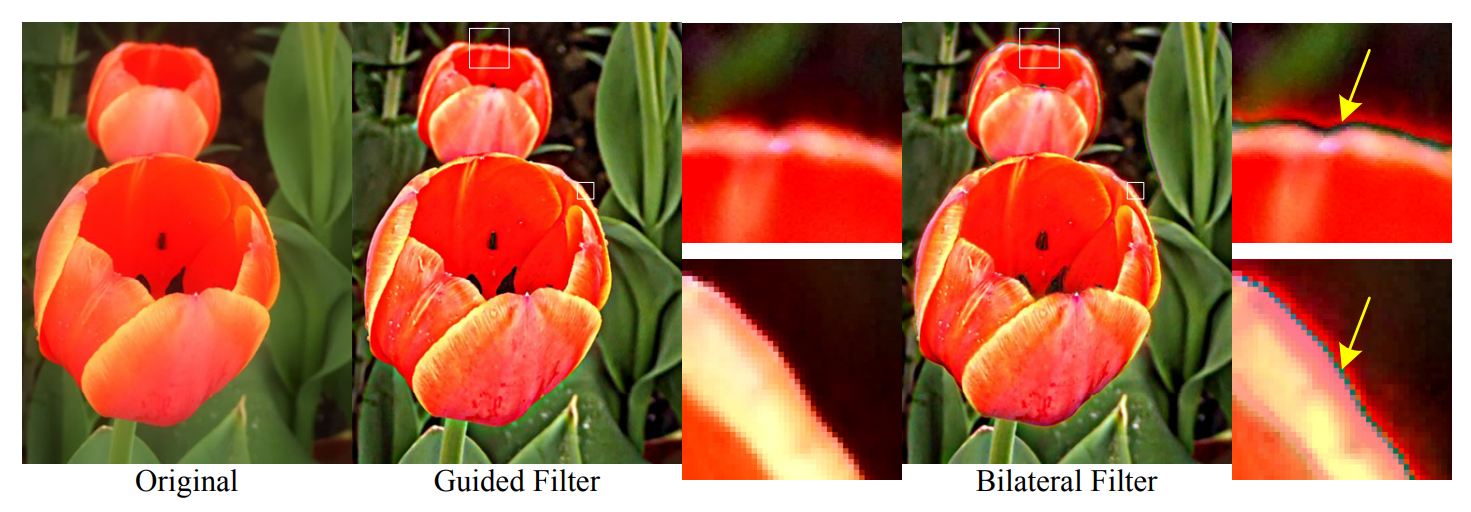
\includegraphics[width=\linewidth]{hw2_1_4}
    \caption{detail-enhanced result of bilateral filter and guided filter.
    $\sigma_s=16$, $\sigma_r=0.1$ is used for bilateral filter, whereas 
    $r=16$ and $\epsilon=0.1^2$ is used for guided filter}
    \label{fig:4}
\end{figure}

Another good property of the above equation is that $\bigtriangledown q$ can be approximated
as a scaling of $\bigtriangledown I$ only when big intensiy change causes small value for
$\bigtriangledown \bar{a_i}$, $\bigtriangledown \bar{b_i}$ where
$\bar{a_i} = 1/|\omega|\sum_{k \in \omega_i}a_k$ and 
$\bar{b_i} = 1/|\omega|\sum_{k \in \omega_i}b_k$. By assuring scaling relation only on edge,
unlike bilateral filter, which gets confused when trying to smooth edge component, gets stable on
the edge and prevents gradient reversal problem.  
Visual representation of gradient preserving property in the guided filter can 
be found in \figurename{\ref{fig:1}}.
Actual result, \figurename{\ref{fig:4}}, also shows that gradient reversal effect is diminished by 
applying guided filter rather than bilateral filter.

\begin{figure}[h]
    \centering
    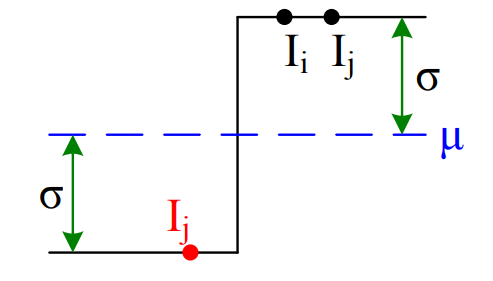
\includegraphics[width=0.3\linewidth]{hw2_1_3}
    \caption{relation between $W_{ij}$ and the directions of $I_i$, $I_j$}
    \label{fig:3}
\end{figure}

From the equation above, the output can be also defined as a linear transformation of the input.
\[q_i = \sum_{j}W_{ij}(I)p_j\]
\[W_{ij}(I) = 1/|\omega|^2\sum_{k:(i,j) \in \omega_k}(1 + \frac{(I_i - \mu_k)(I_j - \mu_k)}{\sigma_k^2 + \epsilon})\]

This form gives a good intuition about edge-preserving property of the guided filter;
As in \figurename{\ref{fig:3}}, when $I_i$ and $I_j$ are on the other side of an edge, 
then $(I_i-\mu_k)(I_j-\mu_k)$ becomes negative, 
thus $(1 + \frac{(I_i - \mu_k)(I_j - \mu_k)}{\sigma_k^2 + \epsilon})$ gets close to zero,
resulting small $W_{ij}$ value. Semantically, small $W_{ij}$ means that 
pixels positioned on $p_i$ and $p_j$ are not smoothed on a scale.
Contrastly, when $I_i$ and $I_j$ are on the same side
of an egde, $(I_i-\mu_k)(I_j-\mu_k)$ becomes positive, making $W_{ij}$ reasonably big
value to smooth the pixels positioned on $p_i$ and $p_j$.

\begin{figure}[h]
    \centering
    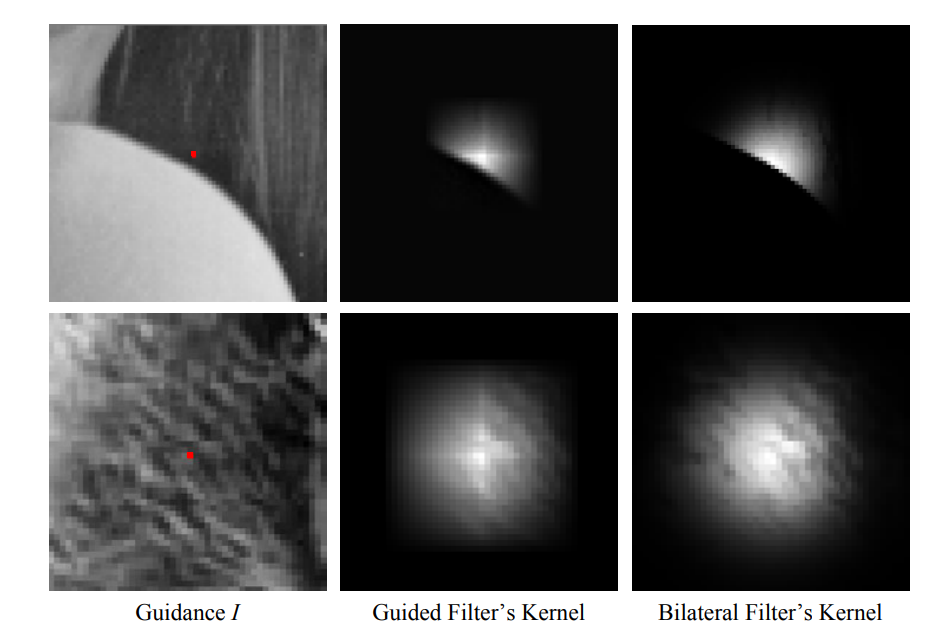
\includegraphics[width=0.8\linewidth]{hw2_1_5}
    \caption{kernel values of guided filter/bilateral filter in various guide image}
    \label{fig:5}
\end{figure}

\figurename{\ref{fig:5}} contains kernel values of both guided filter and bilateral filter.
On top guide image, it can be also seen that on both bilateral filter and guided filter, 
kernel is constructed as to preserve dominant edge (dividing bottom and top diagonally).
Guidance image having less dominant edge incurs both bilateral filter and guided filter
to have omnidirectional smoothing effect.

As discussed above, guided filter assumes linear transformation from guidance to input 
and aggregate the guide-transformed output within a window. This can prevent the
occurence of gradient reversal problem with time complexity of O(N).
Guided filter can be applied in various fields of image processing, including detail
enhancement, denoising, matting, haze removal and so forth.

\pagebreak
\subsection*{problem 1: rolling guidance filter}

Rolling guidance filter \cite{rolling} is a scale-aware local operation filter that controls smoothing
details with a scale measure, by which small-scale structures can be removed while preserving others.
Despite of its simple implementation, it can be run with various types of guidance filters, and 
converges within several steps of iteration.

\begin{figure}[h]
    \centering
    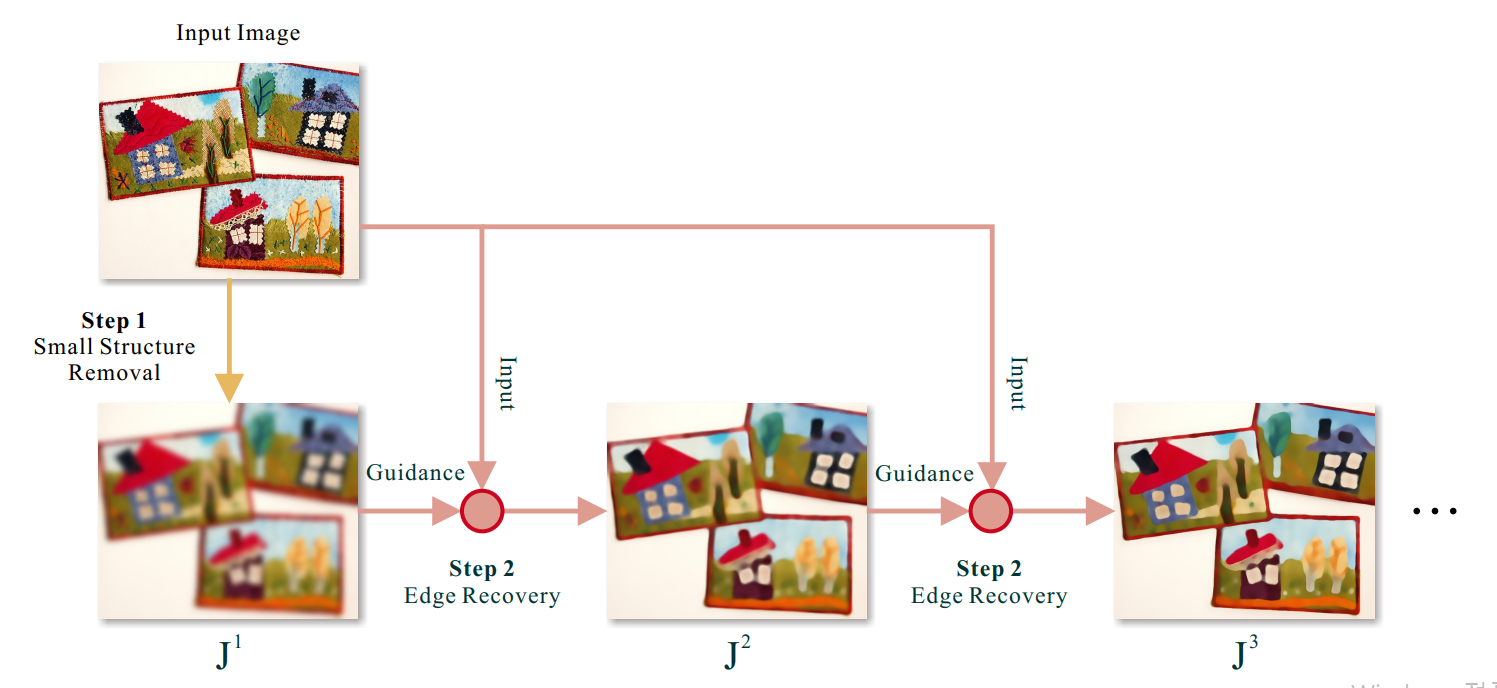
\includegraphics[width=\linewidth]{hw2_1_6}
    \caption{flow diagram of rolling guidance filter}
    \label{fig:6}
\end{figure}

Rolling guidance filter consists of two steps; small structure removal and 
edge recovery (\figurename{\ref{fig:6}}).
At beginning, gaussian filter is used to remove small structures, which also involves blurring at
large-scale intensity variations.
\[G(p) = 1/K_p\sum_{q \in N(p)}exp(-\frac{||p-q||^2}{2\sigma_s^2})I(q)\]
\[K_p = \sum_{q \in N(p)}exp(-\frac{||p-q||^2}{2\sigma_s^2})\]
where $K_p$ is the normalization term and $N(p)$ stands for the set of neighboring pixels of $p$.
The next edge recovery step iteratively recovers edge with joint bilateral filter, with the guidance
image as its previous step output. $J^t$ stands for the recovery result from the $t$-th iteration.
It can also be possible to use other types of edge-recovery filter such as guided filter.
\[J^{t+1}(p) = JointBilateral(p, I, J^t, \sigma_s, \sigma_r)\]
\[= 1/K_p\sum_{q \in N(p)}exp(-\frac{||p-q||^2}{2\sigma_s^2}-\frac{||J^t(p)-J^t(q)||^2}{2\sigma_r^2})I(q)\]
\[K_p = \sum_{q \in N(p)}exp(-\frac{||p-q||^2}{2\sigma_s^2}-\frac{||J^t(p)-J^t(q)||^2}{2\sigma_r^2})\]

When using joint bilateral filter as its guidance, the small structure removal
step and the edge recovery step can be merged if $J^0$ is a constant-value image. 
Assign $J^t$ as a constant $C$, then the resulting $J^t$ has the form exactly 
same as gaussian filter. The combined iteration is described in Algorithm 1.
\[J^t(p) = C \forall p\]
\[J^{t+1}(p) = 1/K_p\sum_{q \in N(p)}exp(-\frac{||p-q||^2}{2\sigma_s^2}-\frac{||J^t(p)-J^t(q)||^2}{2\sigma_r^2})I(q)\]
\[= 1/K_p\sum_{q \in N(p)}exp(-\frac{||p-q||^2}{2\sigma_s^2})I(q) = G(p)\]

\begin{algorithm}
    \caption{rolling guidance filter}
    $J^0 \gets$ constant image\;
    \For{$t = 1:num\_iter$}{
        $J^t \gets joint\_bilateral(I, J^{t-1}, \sigma_s, \sigma_r)$\;
    }
    return $J^{num\_iter}$\;
\end{algorithm}

\begin{figure}[h]
    \centering
    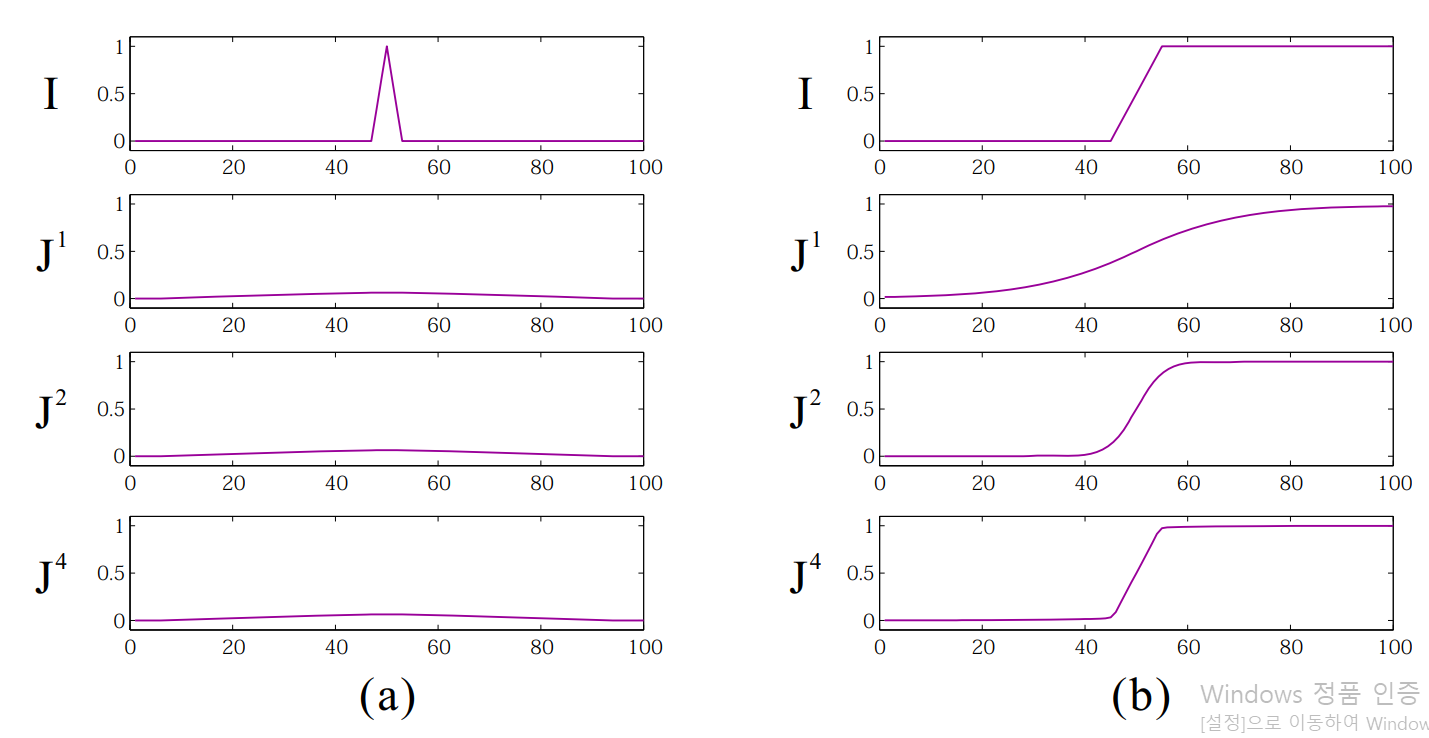
\includegraphics[width=\linewidth]{hw2_1_2}
    \caption{iteration result $J^t$ in 1-D signal. (a) small structure 
    (b) large structure, edge component}
    \label{fig:2}
\end{figure}

\begin{figure}[h]
    \centering
    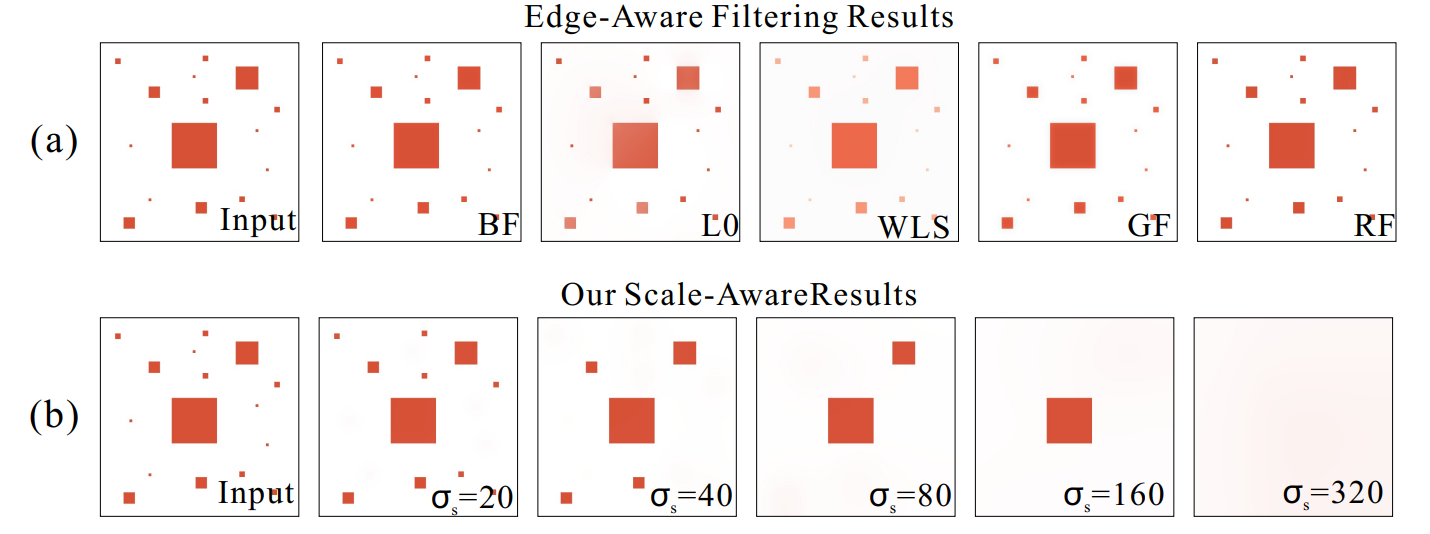
\includegraphics[width=\linewidth]{hw2_1_8}
    \caption{comparison on edge-aware filtering (bilateral, $L^0$, WLS, guided, recursive filters) 
    and scale-aware filtering (rolling guidance filter)}
    \label{fig:8}
\end{figure}

The detailed iteration process and its output in 1-D signal example and the real image can be
found from \figurename{\ref{fig:2}}, \figurename{\ref{fig:7}} respectively.
As the iteration progresses, small structure smoothes out ($I$ to $J_1$ from 
\figurename{\ref{fig:2}} (a)) while large structure gets blurred
at the first phase and then the edge is recovered.
Intermediate results on iterative edge recovery phase (\figurename{\ref{fig:7}}) also indicates 
the average number of iterations needed for the final output. It can be seen that in the
specific image, within 10 iterations the edge is almost recovered.

\begin{figure}[h]
    \centering
    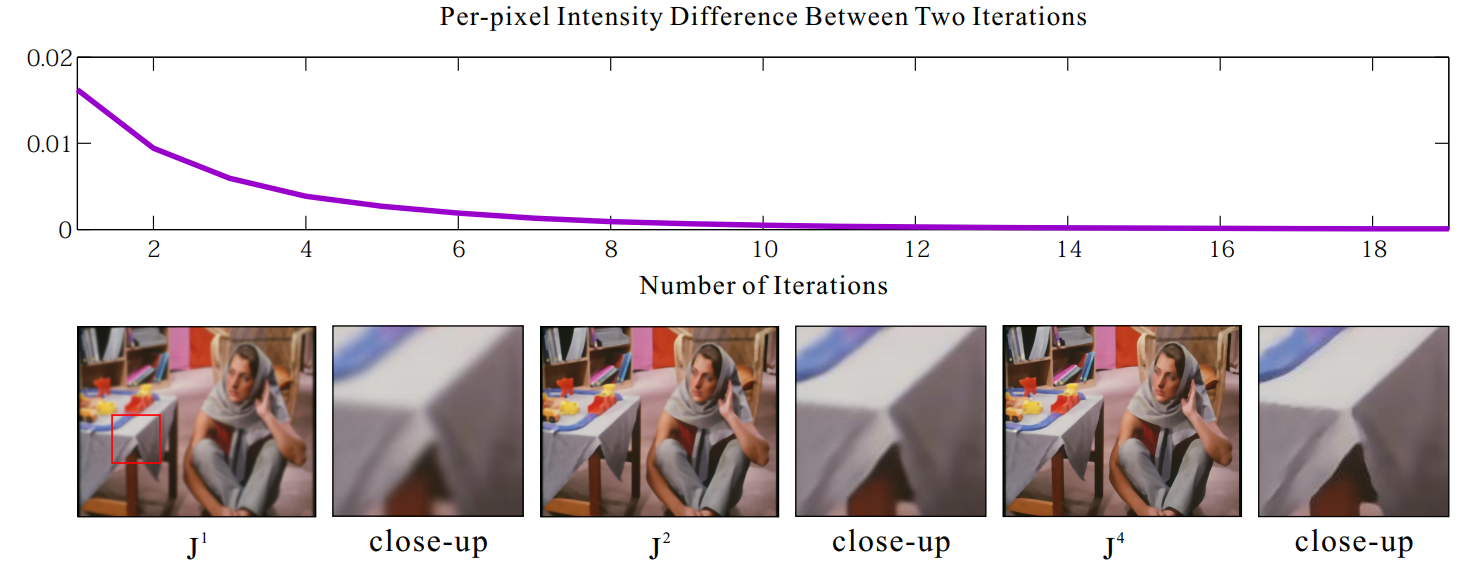
\includegraphics[width=\linewidth]{hw2_1_7}
    \caption{output image $J_t$ on different timestep}
    \label{fig:7}
\end{figure}

\figurename{\ref{fig:8}} shows the scale-aware nature of the rolling guidance filter.
It can be seen the existing edge-aware filtering cannot successively remove the small scale
elements while preserving the large scale element as it is, while in rolling guidance filter
depending on $\sigma_s$ the elements are masked out in the order of their scales. 

Due to its simple implementation with fast and reasonably good result on scale-aware
filtering, many applications can earn benefit from the rolling guidance filter; including
detail enhancement, tone mapping, multi-scale structure decomposition, segmentation
and so on. Especially, virtual contour restoration characteristic of the filter can
boost performance on segmentation task by providinf large-scale image information.

\pagebreak
\subsection*{problem 2: cross image filtering}

hw2\_2.m reads input, guidance image and apply both joint bilateral filter and guided filter.
input image, art\_depth\_low\_res.png contains low resolution depth image, 
and guidance image, art\_color\_high\_res.png
contains high resolution color image. The goal of applying the filters onto the images
is to increase edge details within the depth image by utilizing color image as its
guidance.

\begin{figure}[h]
    \centering
    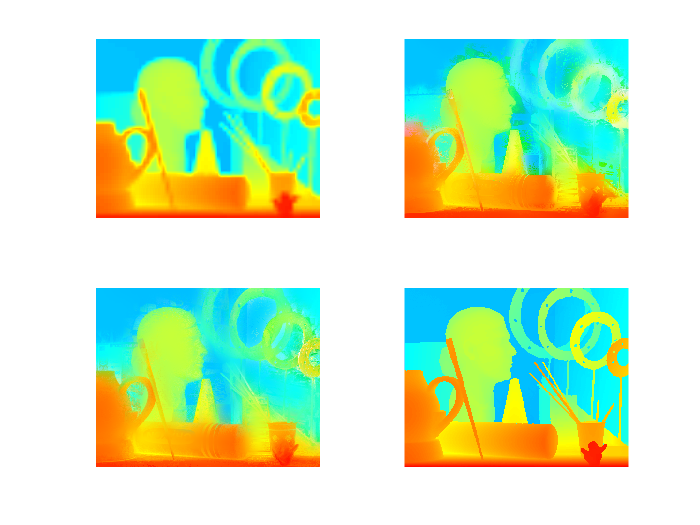
\includegraphics[width=\linewidth]{hw2_2_1}
    \caption{result of hw2\_2.m. top left : original input image,
    top right : output of joint bilateral filter with kernel diameter 65,
    both $\sigma_s$ and $\sigma_r$ 10,
    bottom left : output of guided filter with kernel diameter = 65, $\epsilon = 4e-1$,
    bottom right : ground truth high resolution image}
    \label{fig:9}
\end{figure}

\figurename{\ref{fig:9}} shows the result of applying both filter given input and guidance image.
It can be seen that in both joint bilateral and guidance filter, the details on edge components
are boosted. However, no discrete segmentation could be achieved like in the groundtruth image
from both filters. That would be partially due to the intensity variance of the guidance image.
Flattening guidance image to have less textual or small scaled variation might help in the case.

Pseudocode for joint bilateral and guided filters are as follows. It can be seen that
the complexity of joint bilateral filter and guided filter is O($Nr^2$) and O(N) respectively 
where $N$ is the size of input image and $r$ is kernel radius (In the pseudocode of guided filter,
extracting mean from each window is described; vanilla implementation will require O($r^2$) computation,
but this can be achieved in constant time by the integral technique):

\begin{algorithm}
    \caption{joint\_bilateral.m}
    $pad_{i} \gets pad(input, radius)$\;
    $pad_{g} \gets pad(guidance, radius)$\;
    $gauss\_range \gets gauss(radius, \sigma_s)$\;
    
    \For{$i = 1:M$}{
        \For{$j = 1:N$}{
            $window_{i} \gets pad\_input(i:i+2*radius, j:j+2*radius)$\;
            $window_{g} \gets pad\_guidance(i:i+2*radius, j:j+2*radius)$\;
            $gauss\_spatial \gets exp(-(window_{i}(i,j)-guidance(i,j))^2/(2*\sigma_r^2))$\;
            \For{$k = 1:C$}{
                $denom \gets sum(gauss\_range * gauss\_spatial)$\;
                $output(i,j,k) \gets sum(gauss\_range * gauss\_spatial * window_{i}) / denom$\;
            }
        }
    }
\end{algorithm}

\begin{algorithm}
    \caption{guided.m}
    pad $input$, $guidance$ into $pad_{i}$, $pad_{g}$\;
    calculate $\mu_{g}$, $\sigma_{g}$\;

    $a, b \gets zeros$\;
    \For{$i = 1:M$}{
        \For{$j = 1:N$}{
            \For{$k = 1:C$}{
                extract $window_{g}$ and $window_{i}$\;
                $a(i,j,k) = mean(window_{g} * window_{i} - \mu_{g}(i,j,k) * mean(window_{i}))$\;
                $a(i,j,k) = a(i,j,k) / (\sigma_{g}(i,j,k) + \epsilon)$\;
                $b(i,j,k) = mean(window_{i}) - a(i,j,k) * \mu_{g}(i,j,k)$\;
            }
        }
    }
    
    pad $a$, $b$ into $pad_{a}$, $pad_{b}$\;
    \For{$i = 1:M$}{
        \For{$j = 1:N$}{
            \For{$k = 1:C$}{
                extract $window_{a}$ and $window_{b}$\;
                $output(i,j,k) = mean(window_{a} * guidance(i,j,k) + window_{b})$\;
            }
        }
    }
\end{algorithm}

\subsection*{problem 3: texture removal}

hw2\_3.m reads image.png, apply rolling guidance filter with both joint bilateral filter
and guided filter. The result can be found in \figurename{\ref{fig:10}}.

In \figurename{\ref{fig:10}}, the leftmost images on both top and bottom are result of 
applying gaussian filter on the original image. It can be seen that both small structures like
texture of table are smoothed out while large structures like table corder are
blurred. As iteration proceed, large scale edge components are gradually restored.

\begin{figure*}[h]
    \centering
    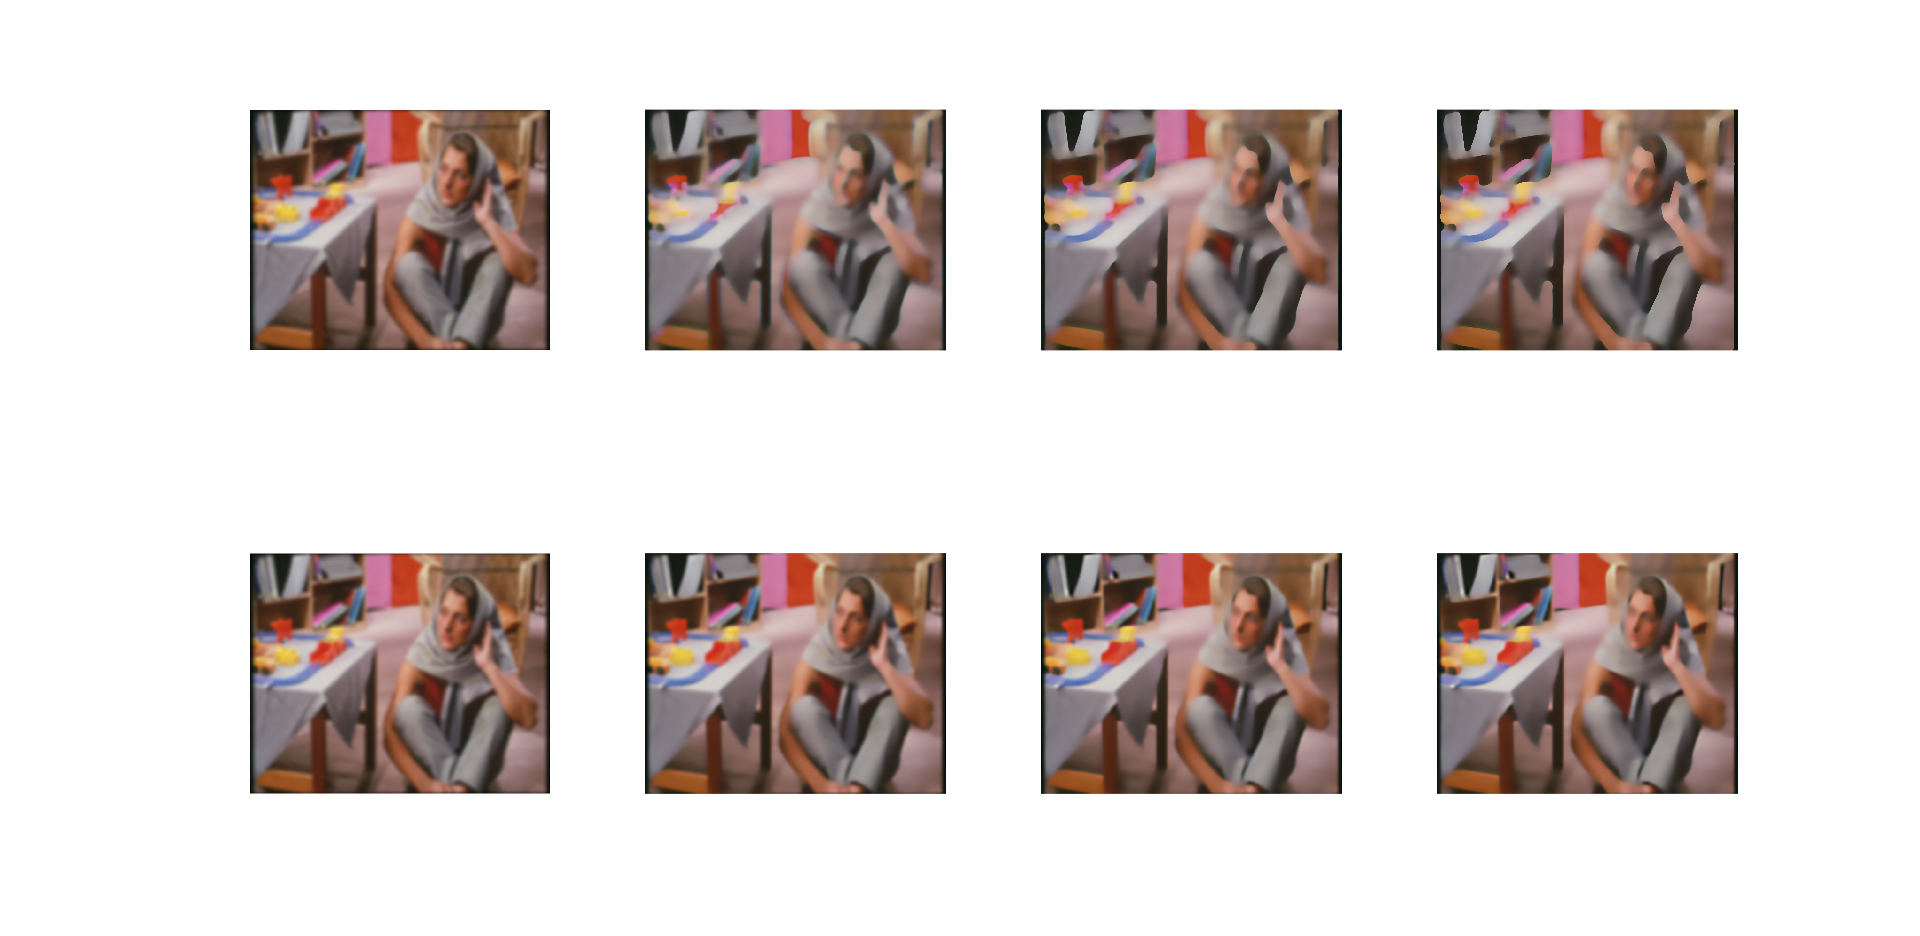
\includegraphics[width=\linewidth]{hw2_3_1}
    \caption{result of hw2\_3.m. top : joint bilateral filter as guidance for
    rolling guidance, bottom : guided filter as guidance for rolling guidance.
    From left to right, each image stands for $J^1$, $J^2$, $J^4$ and $J^6$
    intermediate output}
    \label{fig:10}
\end{figure*}

\subsection*{problem 4: WLS filter}

hw2\_4.m reads noisy\_image.png and apply bilateral, guided and WLS filter. 
\figurename{\ref{fig:11}} depicts the result of applying various filter onto the noisy input. 
It can be seen that both three filters can remove noise in some amount, but their 
edge preserving status is different. In bilateral filter output, edges are blurred In
great amount. Though this edge smoothing effect is alleviated on guided filter, it also
contains some blurring effect. On WLS result, while suppressing noisy componenet, most of 
edge components are successively preserved.

\begin{figure*}[h]
    \centering
    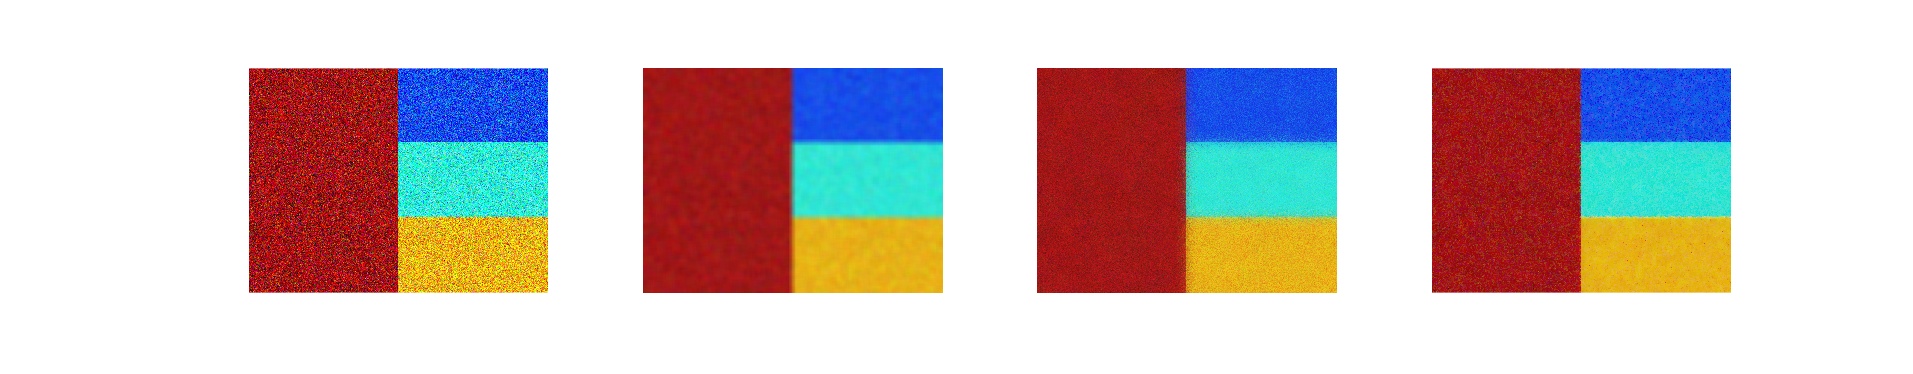
\includegraphics[width=\linewidth]{hw2_4_1}
    \caption{result of hw2\_4.m. left : original image, second : output of bilateral filter 
    with kernel size = 5, $\sigma_s$ = 5, third : output of guided filter with guidance as
    itself, kernel diameter = 17 and $\epsilon$ = 1e-1, fourth : output of WLS filter with
    $\lambda$ = 2, $\alpha$ = 1.2 and $\epsilon$ = 1e-4}
    \label{fig:11}
\end{figure*}

Pseudocode for WLS filter implementation is as below. Efficient calculation of 
Laplacian matrix could be achieved by the sparse matrix.

\begin{algorithm}
    \caption{wls.m}
    $dl\_dx \gets diff(log(input), 1, 2)$\;
    $a_x \gets 1 / (abs(dl\_dx)^\alpha + \epsilon)$\;
    flatten $a_x$\;
    $a_x\_shift \gets shift(a_x, M)$\;

    $dl\_dy \gets diff(log(input), 1, 1)$\;
    $a_y \gets 1 / (abs(dl\_dy)^\alpha + \epsilon)$\;
    flatten $a_y$\;
    $a_y\_shift \gets shift(a_y, 1)$\;

    $L_g\_diag \gets a_x + a_x\_shift + a_y + a_y\_shift$\;
    build sparse diagonal matrix $L_g$ with diagonal element $-a_x$, $-a_y$ and $L_g\_diag$\;
    $lhs \gets I + \lambda * L_g$\;

    solve $lhs * u = input$ linear equation\;
\end{algorithm}

\subsection*{references}

\begin{thebibliography}{9}
    \bibitem{guided}
    He, Kaiming, Jian Sun, and Xiaoou Tang. "Guided image filtering." 
    IEEE transactions on pattern analysis and machine intelligence 35.6 (2012): 1397-1409.
    
    \bibitem{rolling}
    Zhang, Qi, et al. "Rolling guidance filter." European conference on computer vision. Springer, Cham, 2014.
\end{thebibliography}

\end{document}
